\documentclass[tikz, border=20pt]{standalone}
\usepackage{amsmath, amssymb}
\usepackage{xcolor}
\usetikzlibrary{decorations.pathreplacing, positioning, calc, shapes.geometric}

\begin{document}
	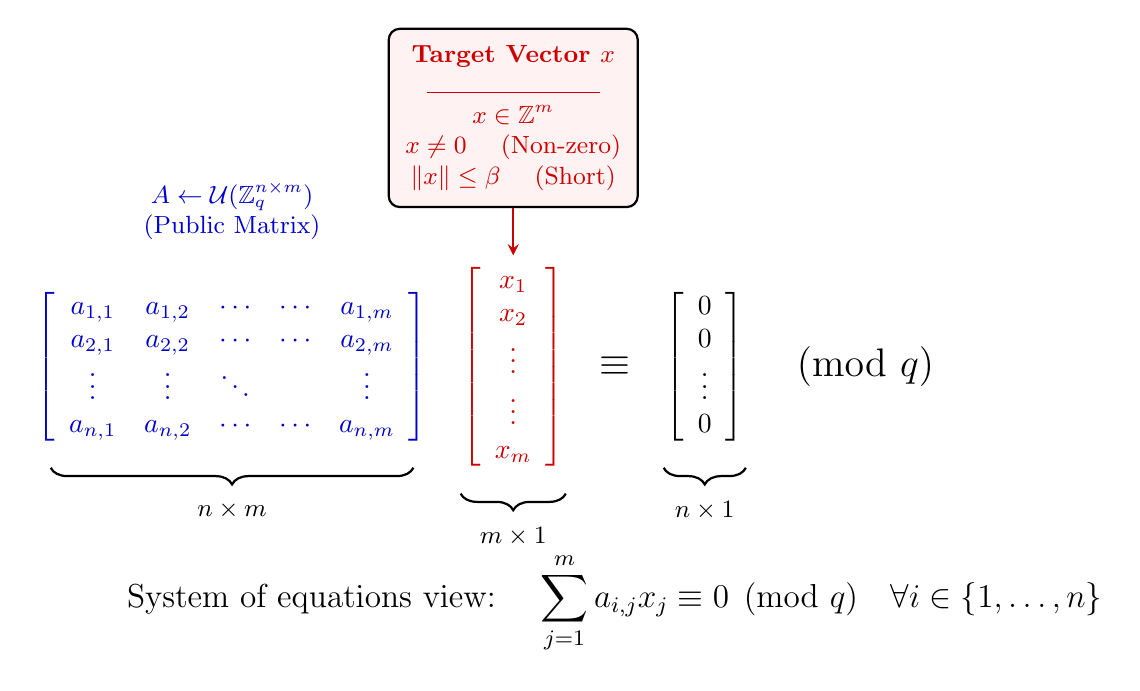
\begin{tikzpicture}[
		>=stealth,
		public/.style={text=blue!80!black},
		secret/.style={text=red!80!black},
		annotation/.style={font=\small, align=center}
		]
		
		% ==========================================
		% MATRIX A (Public)
		% ==========================================
		\node[public] (A) {
			$\left[
			\begin{array}{ccccc}
				a_{1,1} & a_{1,2} & \cdots & \cdots & a_{1,m} \\
				a_{2,1} & a_{2,2} & \cdots & \cdots & a_{2,m} \\
				\vdots  & \vdots  & \ddots & & \vdots  \\
				a_{n,1} & a_{n,2} & \cdots & \cdots & a_{n,m}
			\end{array}
			\right]$
		};
		
		% ==========================================
		% VECTOR x (Target / Short)
		% ==========================================
		\node[secret, right=0.2cm of A] (x) {
			$\left[
			\begin{array}{c}
				x_1 \\ x_2 \\ \vdots \\ \vdots \\ x_m
			\end{array}
			\right]$
		};
		
		% Equals Sign
		\node[right=0.2cm of x, font=\Large\bfseries] (eq) {$\equiv$};
		
		% ==========================================
		% VECTOR 0 (Target Output)
		% ==========================================
		\node[right=0.2cm of eq] (zero) {
			$\left[
			\begin{array}{c}
				0 \\ 0 \\ \vdots \\ 0
			\end{array}
			\right]$
		};
		
		% Modulo
		\node[right=0.2cm of zero, font=\Large] (mod) {$\pmod q$};
		
		% ==========================================
		% DIMENSION BRACES
		% ==========================================
		\draw[decorate,decoration={brace,amplitude=6pt,mirror}, thick]
		([yshift=-0.2cm, xshift=0.3cm]A.south west) -- ([yshift=-0.2cm, xshift=-0.3cm]A.south east) 
		node[midway, below=0.3cm, font=\small] {$n \times m$};
		
		\draw[decorate,decoration={brace,amplitude=6pt,mirror}, thick]
		([yshift=-0.2cm, xshift=0.1cm]x.south west) -- ([yshift=-0.2cm, xshift=-0.1cm]x.south east) 
		node[midway, below=0.3cm, font=\small] {$m \times 1$};
		
		\draw[decorate,decoration={brace,amplitude=6pt,mirror}, thick]
		([yshift=-0.2cm, xshift=0.1cm]zero.south west) -- ([yshift=-0.2cm, xshift=-0.1cm]zero.south east) 
		node[midway, below=0.3cm, font=\small] {$n \times 1$};
		
		% ==========================================
		% LABELS & CONSTRAINTS
		% ==========================================
		\node[above=0.4cm of A, public, annotation] {$A \leftarrow \mathcal{U}(\mathbb{Z}_q^{n \times m})$ \\ (Public Matrix)};
		
		% Highlight box for the conditions on x
		\node[above=0.6cm of x, secret, draw, thick, rounded corners, fill=red!5, inner sep=6pt, annotation] (constraints) {
			\textbf{Target Vector $x$}\\
			\rule{2.2cm}{0.4pt}\\
			$x \in \mathbb{Z}^m$\\
			$x \neq 0$ \quad (Non-zero)\\
			$\|x\| \le \beta$ \quad (Short)
		};
		\draw[->, thick, red!80!black] (constraints.south) -- (x.north);
		
		% ==========================================
		% LINEAR SYSTEM ANNOTATION
		% ==========================================
		\node[below=2cm of eq, font=\large] (system) {
			System of equations view: \hspace{0.2cm} 
			$\displaystyle \sum_{j=1}^{m} a_{i,j} x_j \equiv 0 \pmod q \quad \forall i \in \{1, \dots, n\}$
		};
		
	\end{tikzpicture}
\end{document}